So far I have demonstrated that it is possible to design a type system for most
of real-world C. In particular, such a type system supports resource management
in the presence of complex control flow, variable scoping and aliasing, and has
a conceptually simple extension to handle loose evaluation order.

One of the features I glossed over was the subtle and complex rules regarding
pointer manipulations, which cannot be ignored or simplified away in practice,
especially given \kl{CN}'s headline goal (\cref{sec:cn-intro}) to work
correctly above pre-existing C programs and observed behaviour.

The subtlety around observed behaviour for pointer manipulations stems from the
competing forces which shaped C.\sidenote{Inherited portability requirements,
proximity to hardware, and the desire for more aggressive optimisations.} As I
explained in \cref{sec:c-lang}, a completely concrete view of pointers would
invalidate fundamental optimisations we would like to perform on our code, but
a completely abstract view where pointers cannot alias each other is simply
incompatible with C's ability to take addresses of variables and compute with
pointers (incremet, calculate offsets, cast them to and from integers).

Whilst many aspects of C are specified using an elaboration, the representation
of pointers, and the choice of rules for manipulating them, are factored out
into a \emph{memory interface}. This interface is visible in
\cref{fig:effectful-core-grammar}: the memory operations $\mathit{memop}$ and
the memory $\mathit{actions}$; a \intro{memory object model}\sidenote{Named so
to distinguish it from a memory model in a concurrency setting.} is an
implementation of that interface.

Remember that C has a lot of different stakeholders, and so a memory model
which is acceptable to the standards committee needs to walk a fine line
between being concrete enough to enable as many low-level idioms as possible,
whilst being abstract enough to permit as many optimisations as possible. The
key concept which enables this is the idea of pointer \intro{provenance},
tracking where a pointer came from. With this, because C allows casting to and
from integers, the question naturally arises about whether this provenance
should be tracked via integers or not. Unfortunately, that is not the only
choice point involved in coming up with an acceptable memory object model;
\sidetextcite{memarian2022cerberus} documents and explains the trade-offs
between this and other choices.

Any set of choices must nagivate the tension between allowing
low-level idioms relied upon by existing code, allowing opportunities for
optimisations exhibited by existing compilers, and limiting the scope of both.
The cost of doing so (in a consistent manner\sidenote{None of the memory models
discussed are consistent with all observed behaviour, and it is not clear that
there is a consistent one which would be.}) is that the so far preferred (but
not yet officially adopted) memory object model,
\kl{PNVI-ae-udi},\sidenote{Provenance not tracked via integers, for addresses
which are exposed and provenances user-disambiguated. I will explain this imminently.} is a
complex minefield of \kl{UB} no human should be expected to navigate
unassisted.

\kl{PVNI-ae-udi} is complex enough that even implementing it in a C
verification tool is undesirable, especially because in that context, it is
reasonable to place a small extra burden of annotation on the user if it
simplifies verifying the code. This is the motivation behind the development of
\kl{VIP},\sidecite{lepigre2022vip} a memory model which is sound with respect
to PNVI-ae-udi,\sidenote{Quoting from the paper, ``every PNVI-ae-udi step can
be simulated by a VIP step, and that every step that raises
\kl[UB]{undefined behaviour} in PNVI-ae-udi also raises \kl[UB]{undefined
behaviour} in VIP.''} but simpler (it is fine to reject more programs, i.e.\
have more \kl{UB}).

\kl{VIP} as a memory model is \emph{simpler}, but it is not trivial. It is
defined operationally as a step relation between concrete (i.e.\ not symbolic)
heavily structured heaps, and the steps have complex premises.

In this part, I will detail the challenges and choices I faced in designing,
formalising and implementing \kl{CN-VIP}, the memory model of \kl{CN} as a scheme
within the formalised and implemented type systems.
\begin{itemize}
    \item \textbf{Expressiveness vs simplicity.} \kl{VIP} makes a particular
        choices about its representation of pointers and integers, and relatedly
        about the idioms it supports. I will explain it, and the other
        design around it, both simpler and more expressive. In particular,
        I will explain important and subtle complexities around round-trip casts,
        \cinline{memcpy} and \cinline{memcmp}, which are handled in
        \kl{VIP}/\kl{PNVI-*} test-suite, but not discussed.
    \item \textbf{Integration into \kl{Kernel CN}.} As I mentioned in
        \cref{sec:res-terms}, the novel structure for heaps abstracts away
        some aspects of its representation. I will explain how I adapted the
        static and dynamic semantics to use \kl{VIP}, and proved the new system
        sound with less repeated effort than typical.
    \item \textbf{Implementation in \kl{CN}.} I will explain how I incrementally
        developed, gated and deployed a complex change to memory model of \kl{CN}.
        By the time I had designed and formalised \kl{CN-VIP}, \kl{CN} had
        users, a tutorial, a test-suite and a continuous integration pipeline,
        so I had to be careful in adding support for \kl{VIP}, avoid difficult
        code merges and test updates.
    \item \textbf{Impact on annotations and performance.} Finally, I will explain
        how switching over to \kl{CN-VIP} (without round-trip casts) impacted
        the annotations and performance on existing \kl{CN} tests and tutorial
        examples.
\end{itemize}

\chapter{Memory Object Models, explained}\label{chap:mem-model-explained}

\margintoc%

From the perspective of \kl{Core} and \kl{ResCore}, the memory object model
(\cref{fig:mem-model-intf}) is simply a choice of representation of pointers,
and the interface specified in the memory operations $memop$, and memory
$\mathit{actions}$.\sidenote{Plus some extra primitives to detect races between
unsequenced expressions, which I will ignore.}

\begin{marginfigure}
    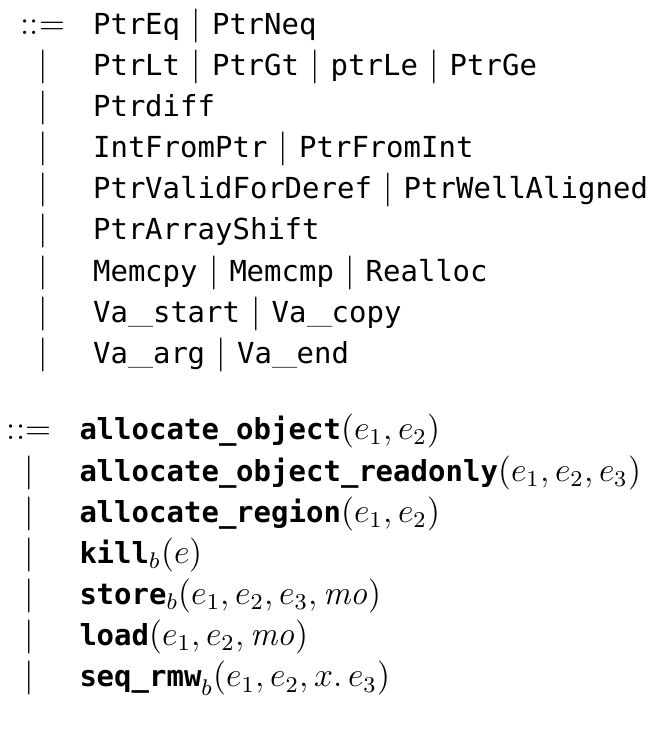
\includegraphics{figures/mem-model-intf}
    \caption{Memory model interface of \kl{Core}.}\label{fig:mem-model-intf}
\end{marginfigure}

The key concept which begins this brief overview of memory object models is
that of provenance. To optimise our code, compilers would like to assume that
not all pointers that a programmer can magically create (a) are valid, i.e.\
point to a live allocation (b) can alias any other live allocation in scope.

Let us revisit the example from \cref{fig:ptr-from-int}, reproduced in
\cref{fig:mem-model-ptr-from-int} for convenience. It shows a simple function
which takes an integer as an argument, assigns the number 5 to a local, and the
prints the value of that local, with some intervening pointer shenanigans.
Despite the fact that there is no data flowing between \cinline{k} and
\cinline{i}, the mere fact that the address of \cinline{j} was taken (and
``exposed'' via its assignment to an integer \cinline{k}) is enough to make the
compiler wary that the pointer \cinline{p} could alias \cinline{j} and thus
disable constant propagation..\sidenote{This example does have \kl{UB} though
because of (demonic) allocation address non-determinism.}

\begin{marginfigure}
    \centering
    \cfile{code/pointer_from_integer_1ie.c}
    \caption{Example pointer\_from\_integer\_1ie.c.}\label{fig:mem-model-ptr-from-int}
\end{marginfigure}

The rules justifying this are set out in the \kl{PNVI-ae-udi} memory model,
upon which VIP is defined. Though the name is clunky and not euphonious, it is
descriptive as each part defines a particular choice to focus on.

\subsection{PNVI\@: provenance not tracked via integers}

For the purposes of defining the dynamic semantics of the memory object model,
each pointer can be thought of as an \emph{pair} of an address $a$ and an
allocation ID $@i$. The address is simply what programmers might be familiar
with as `the pointer', which, unlike the allocation ID, can may inspected or
manipulated directly from the C program at runtime. From the perspective of
separation logic verification, the allocation ID can be thought of the ghost
part of a pointer, but it does play an integral part of the model of memory I
will outline next.

The allocation ID is allocated fresh globally\sidenote{PNVI-ae-udi does not
support concurrency.} for every new allocation, and thus guaranteed to be
unique. An \intro{allocation history} $\mathit{A}$ is a partial map indexed by
allocation IDs, which tracks the size of allocations, base address and whether
or not they are live. The pointer resulting from successfully creating a fresh
allocation is a pair of base address and the allocation ID\@. When an
allocation is destroyed, the entry is not removed, but merely updated to record
the allocation as dead. The allocation history includes other information too,
which I will ignore because it is not relevant to the key concepts.

The \kl{allocation history} merely tracks information about the allocation as a
whole, to track values of what resides in those allocations, \kl{PNVI-ae-udi}
also uses a memory $M$ as part of the abstract state. This is not just a map
from addresses to bytes, but triples of a (potentially empty) provenance and a
concrete 8-bit byte or $\mathsf{unspec}$ value for uninitialised or padding
bytes.\sidenote{There is an additional component, an optional \intro{pointer
    index} (an integer $j$ or $\mathsf{none}$) which stores which part of a
    pointer a byte came from. This is only relevant if either (a) pointer
    values can be stored unaligned (b) pointer types have different sizes or
    (c) provenance is tracked via integers (PVI) and bytes of those pointers
have been overwritten.}\label{sn:ignore-ptr-index}

Reading from and writing to memory is done via the \coreinline{load} and
\coreinline{store} actions, at a specific C type, and these actions handle
structured \kl{Core} values, not sequences of bytes. Marshalling between the
two is handled via $\mathrm{repr}$ and $\mathrm{abst}$ functions. So for
example, a pointer $(a, @i)$ as a value is going to be stored as a sequence of
bytes in memory based on its address $a$, each byte with its provenance
$@i$.\sidenote{There is also an optional \kl{pointer index} for each byte's
position in the pointer, see note~\ref{sn:ignore-ptr-index}.}

One of the idioms existing code relies upon frequently is casting a pointer to
an integer and back again, and this \intro{round-trip} property is in fact
guaranteed by the ISO standard.\sidenote{§6.3.2.3\#5: An integer may be
    converted to any pointer type. Except as previously specified, the result
is implementation-defined, might not be correctly aligned, might not point to
an entity of the referenced type, and might be a trap representation.}. The
most obvious way to assign a provenance to a pointer created from casting an
integer is to simply track the provenance in the integer (PVI) when it was
casted \emph{from} a pointer earlier. However, the updates to the integer
operations to preserve their provenances would break the algebraic properties
of integers relied upon for optimisations by compilers.

Hence the reason for the first crucial design choice in PNVI-ae-udi: the
representation of integer values. As the name suggests, in contrast to PVI,
provenance is not tracked via integers. Casts of integers to pointers therefore
must pick some provenance: a first approximation is to say the result gets the
provenance of an allocation which is live at the time of the cast, whenever the
address is within its footprint.

\subsection{Ae: Considering only address-exposed allocations for round-trips}

Whilst the result of an integer-to-pointer cast getting the provenance of any
live allocation it happens to be contained in is a reasonable choice,
discussions with the standards committee, particularly the memory object model
study group, worried that this would forbid too many non-aliasing assumptions
(required for many optimisations to be applied validly).

A refinement of this approach is to limit the set of considered allocations to
not just the ones which are live, but also the ones which have their addresses
\intro{exposed} (-ae). The \kl{allocation history} would thus also track if an
allocation has been exposed or not, and the semantics of an integer-to-pointer
cast would then only examine those (\cref{fig:pnvi-ival-to-pval}).

\begin{figure*}
    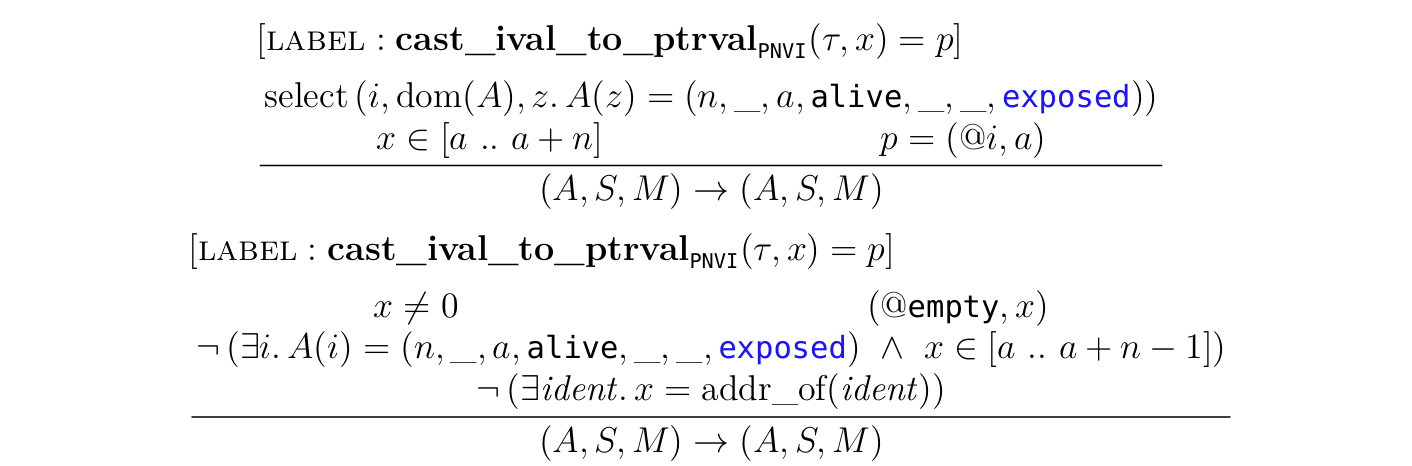
\includegraphics{figures/mem-model-pnvi-ival-to-pval}
    \caption{PNVI-* rules for casting an integer to a pointer. From
    \textcite{memarian2022cerberus}. The first rule should have $x \in [ a \;
        .. \; a + n - 1]$.}\label{fig:pnvi-ival-to-pval}
\end{figure*}

\begin{definition}[Exposed allocation]
An allocation is \emph{exposed} iff a pointer to anywhere within that
allocation
\begin{itemize}
    \item Is cast to an integer.
    \item Has its representation byte read (via a non-pointer lvalue).
    \item Is output via the format specifier \cinline|%p|.
\end{itemize}
\end{definition}

The `within that allocation' is key because one-past pointers (frequently used
to compare against the exclusive end of an allocation) which do not happen to
be that start of an adjacent object would then be assigned an empty provenance
$\mathsf{@empty}$. In turn, this would break the round-trip property required
of casts between pointers and integers for one-past pointers.

\subsection{Udi: disambiguating one-past pointers based on subsequent use}

Restoring round-trip casts for one-past pointers requires an additional
complication to the memory object model, \intro{symbolic} provenances. The
symbolic provenances are mapped to a set of either one or two allocation IDs
via an additional finite map $\mathit{S}$. Thus in the case where an integer
is cast to a one-past pointer on the boundary between two live allocations, its
provenance is assigned to be symbolic, containing both allocations' IDs
(\cref{fig:pnvi-ival-to-pval-symbolic}).

\begin{figure*}
    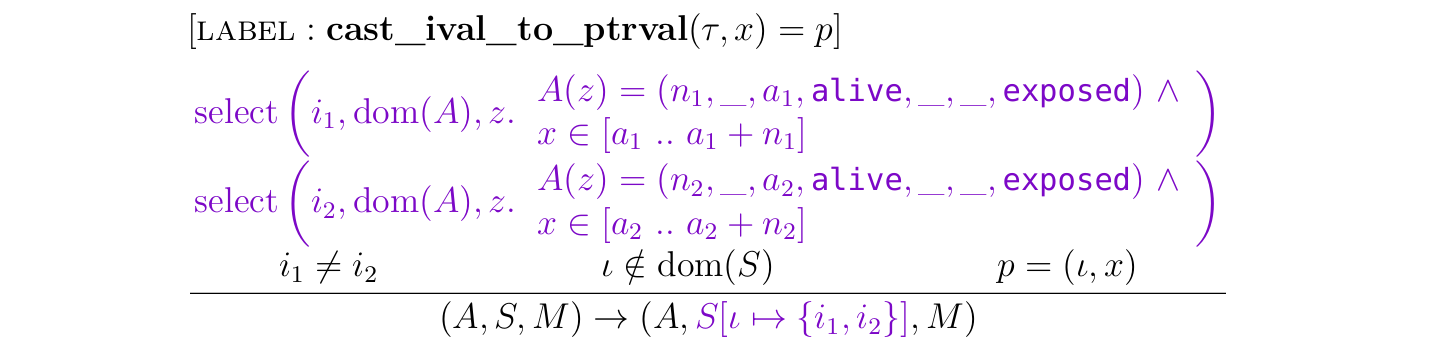
\includegraphics{figures/mem-model-pnvi-ival-to-pval-symbolic}
    \caption{PNVI-ae-udi rule for casting an integer to a pointer when
        the value is the address on the boundary between two live allocations.
        From \textcite{memarian2022cerberus}.}\label{fig:pnvi-ival-to-pval-symbolic}
\end{figure*}

Whilst useful for capturing many idioms and optimisations, the problem with these
symbolic provenances is that they complicate every other rule which requires
knowing the provenance of a pointer, usually to do some liveness and bounds checks.
Furthermore, these provenances can stay symbolic indefinitely, but if disambiguated
by what the user wrote (udi), must remain consistent from then onwards. The
most egregious example of this is the rule for subtracting pointers: there
are \emph{four} cases, \emph{three} of which stem from the existence of symbolic
provenances.
\begin{enumerate}
    \item \textbf{Neither pointer has symbolic provenance.} Both must be within
        bounds of the live allocation signified by their (equal) allocation
        IDs.
    \item \textbf{One pointer has symbolic provenance.} Both pointers must be
        within bounds of the live allocation signified by the concrete
        provenance, which must must be a member of symbolic one; the latter in
        turn is marked as disambiguated.
    \item \textbf{Both pointers have equal symbolic provenances.} Both must
        be within the bounds of either live allocations signified by the
        symbolic provenances, both of which remain ambiguous.
    \item \textbf{Both pointers have symbolic provenances with one in common.}
        Both must be within the bounds of the common live allocation, and
        both their symbolic provenances are marked as disambiguated.
\end{enumerate}

\section{VIP:\ Verified Integer Pointer Casts}

\kl{VIP}, by \sidetextcite{lepigre2022vip}, is a memory object model designed
to be a sound abstraction of PNVI-ae-udi. In particular, it relies on (the
acceptable trade-off of) requiring a small additional annotation burden to
simplify verification. Every \kl{UB}-free VIP program corresponds to a valid
PNVI-ae-udi program, and every \kl{UB} in \kl{PNVI-ae-udi} is also \kl{UB} in
\kl{VIP} (though \kl{VIP} itself may have more \kl{UB} than \kl{PNVI-ae-udi},
achieving its simplicity by increasing its restrictiveness).

\kl{VIP} achieves this by adding a single simplifying restriction on the
round-trip property: only integer values which were cast from pointers, with no
intervening operations, can be round-trip cast back to pointers. Any
intervening operation on that integer (including adding 0) will result in an
$\mathsf{@empty}$ provenance when cast to a pointer.

This restriction is sufficient to remove both \kl{exposure tracking} and
consequently \kl{symbolic provenances} and from the memory model of
\kl{PNVI-ae-udi}. This is because fundamentally VIP tracks exposure of specific
\emph{pointer values} rather than of whole allocations. Disallowing intervening
operations (even if the integer value remains within the bounds of the same
allocation) removes the need to do a search and bounds check of all live
allocation when casting back (I will discuss how \kl{VIP} recovers allocation
IDs in such cases soon). This also means that a boundary pointer is
disambiguated as soon as it is cast back, based on what it was cast from.

This restriction, particularly the `no intervening operation', forbids too
many desirable low-level idioms, such as pointer tagging.\sidenote{Programmers
store information in the lower or upper bits of pointers by exploiting platform
pointer alignment and addressable memory constraints respectively.} To
support these idioms, \kl{VIP} also provides a primitive, called
\cinline[breaklines]{void *copy_alloc_id(uintptr_t, void*)}, which lets a % chktex 36
programmer cast any integer to a pointer (with the appropriate checks).
This primitive is given both a direct semantics above the VIP abstract
state, and a translation into \kl{PNVI-ae-udi}.

The way that both of these are achieved is a very limited form of tracking
provenances via integers. Integer values in VIP model are represented by a
datatype with two constructors: $\mathit{Loc(a, @i)} \mid \mathit{Int(z \in
\mathbb{Z})}$. Casts from pointers $(a, @i)$ to integers just embed the pointer
into the $\mathit{Loc}$ constructor, and casts back to pointers just take the
value out (\cref{fig:vip-ival-to-pval}). If the integer value has any
intervening operations, only the integer parts (the address $a$ in
$\mathit{Loc}$, the payload $z$ in $\mathit{Int}$) are projected and used, any
provenance is forgotten (\cref{fig:vip-arith-binop}). If the integer has no
provenance, then \cinline{copy_alloc_id} can be used to annotate it with one
(\cref{fig:vip-copy-alloc-id}).

\begin{figure*}[tp]
    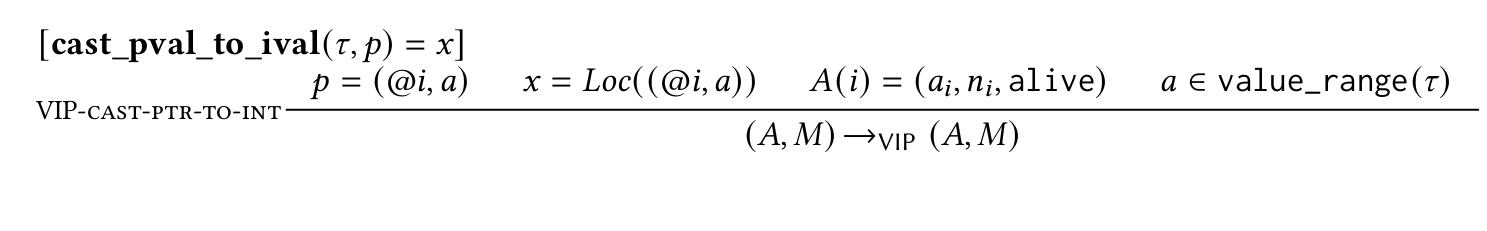
\includegraphics{figures/mem-model-vip-ival-to-pval}
    \caption{The \kl{VIP} rules to cast an integer into a pointer which
    preserves the round-trip property.}\label{fig:vip-ival-to-pval}
\end{figure*}

\begin{marginfigure}
    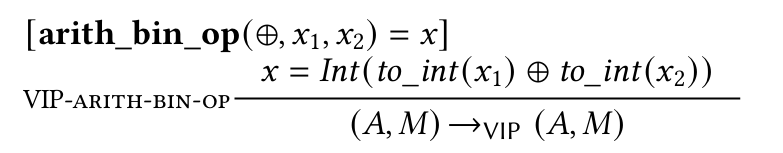
\includegraphics{figures/mem-model-vip-arith-binop}
    \caption{\kl{VIP} arithmetic operations on integers.}\label{fig:vip-arith-binop}
\end{marginfigure}

\begin{figure*}[tp]
    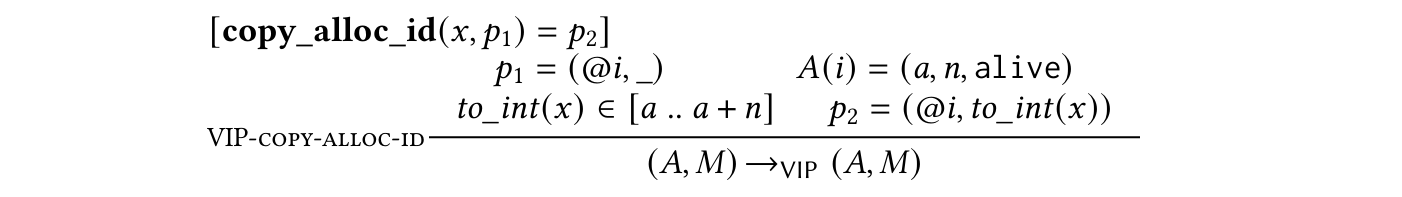
\includegraphics{figures/mem-model-vip-copy-alloc-id}
    \caption{\kl{VIP} \cinline{copy_alloc_id} primitive.}\label{fig:vip-copy-alloc-id}
\end{figure*}

The VIP \cinline{copy_alloc_id} primitive needs to be expressible in
PNVI-ae-udi for it to be a sound abstract, the way this is done is by
essentially implementing it as a C function
(\cref{fig:vip-copy-alloc-id-impl}). The implementation triggers two events in
\kl{PNVI-ae-udi}, the composition of which have the same effect as
\cinline{copy_alloc_id}: it ensures the allocation is \kl{exposed} by casting
it to an integer type, and then casts the integer to the pointer type. There
are some subtleties relating to the fact that the resulting provenance is
always concrete in \kl{VIP} but may be symbolic in \kl{PNVI-ae-udi}, but this
is not an issue because in well-defined programs, they differ only in
\emph{when} the disambiguation takes place (eagerly for \kl{VIP} and lazily for
\kl{PNVI-ae-udi}) rather than which way it disambiguates.

\begin{marginfigure}
    \cfile[breaklines,fontsize=\footnotesize]{code/copy_alloc_id.c}
    \caption{Implementation of \kl{VIP} \cinline{copy_alloc_id} primitive in C, to
        work above existing compilers, modelled via
        \kl{PNVI-ae-udi}.}\label{fig:vip-copy-alloc-id-impl}
\end{marginfigure}


\section{Design space}

Given this background, I will now consider some of the trade-offs involved
expressing different features of \kl{PNVI-ae-udi} and \kl{VIP} in \kl{CN}.

\subsection{Symbolic provenances}

Symbolic provenances initially seem like they should be easy to implement,
especially on top an SMT solver we use to do symbolic execution anyway. Whilst
the rules might be complicated, the potential advantage of not needing further
memory object model related annotations may be significant enough to be worth
it.

However, the symbolic nature of SMT problems turns out to not be helpful or
sufficient by itself to model symbolic provenances. The biggest reason why is
because of \intro{demonic allocation address non-determinism}. This is
orthogonal to \kl{PNVI-ae-udi} and \kl{VIP}, which are defined with respect to
a trace on a specific choice of addresses. It means that a program is deemed to
have \kl{UB} if there exists at least one choice of addresses for allocations
for which the memory object would signal \kl{UB}. In practise, this means that
the C program should not rely on objects being located at pre-determined
addresses or laid out with particular adjacencies, since both of those can be
changed with a different choice of addresses for allocations.

In a symbolic setting, this means an integer cast into an ambiguous one-past
pointer could belong to \emph{any} live allocation, not just one of two as in
the concrete address case.

Another serious problem is that the disambiguation of a provenance is a
\emph{relevant} fact: forgetting this would enable disambiguating the pointer
in inconsistent ways. This means that the disambiguation would need to be
tracked in the (linear) resource context, not the (intuitionistic) constraint
context.

So the choice is between: use annotations to thread pointer disambiguation in
pre- and postcondtions, or use the \cinline{copy_alloc_id} annotation to force
eager disambiguation and sidestep the associated implementation complexity.
I chose the latter.

\subsection{Exposure tracking}

Exposure tracking is another feature that \kl{PNVI-ae-udi} has but \kl{VIP}
does not. Remember that exposure tracking was devised to support round-trip
casts, but restrict the number of aliases which could be considered for the
results of those casts.

Exposure tracking has the distinct advantage over \kl{VIP} that round-trip
casts can happen (a) in the presence of intervening operations on the integer
value and (b) more importantly, \emph{without} a pointer to the specific
allocation we care about being available at runtime.

Are there any idioms which require these two constraints though? And what would
be the associated implementation cost?

Don't forget to mention the byte-level provenance and memcpy!

\begin{figure}[h]
    \centering
    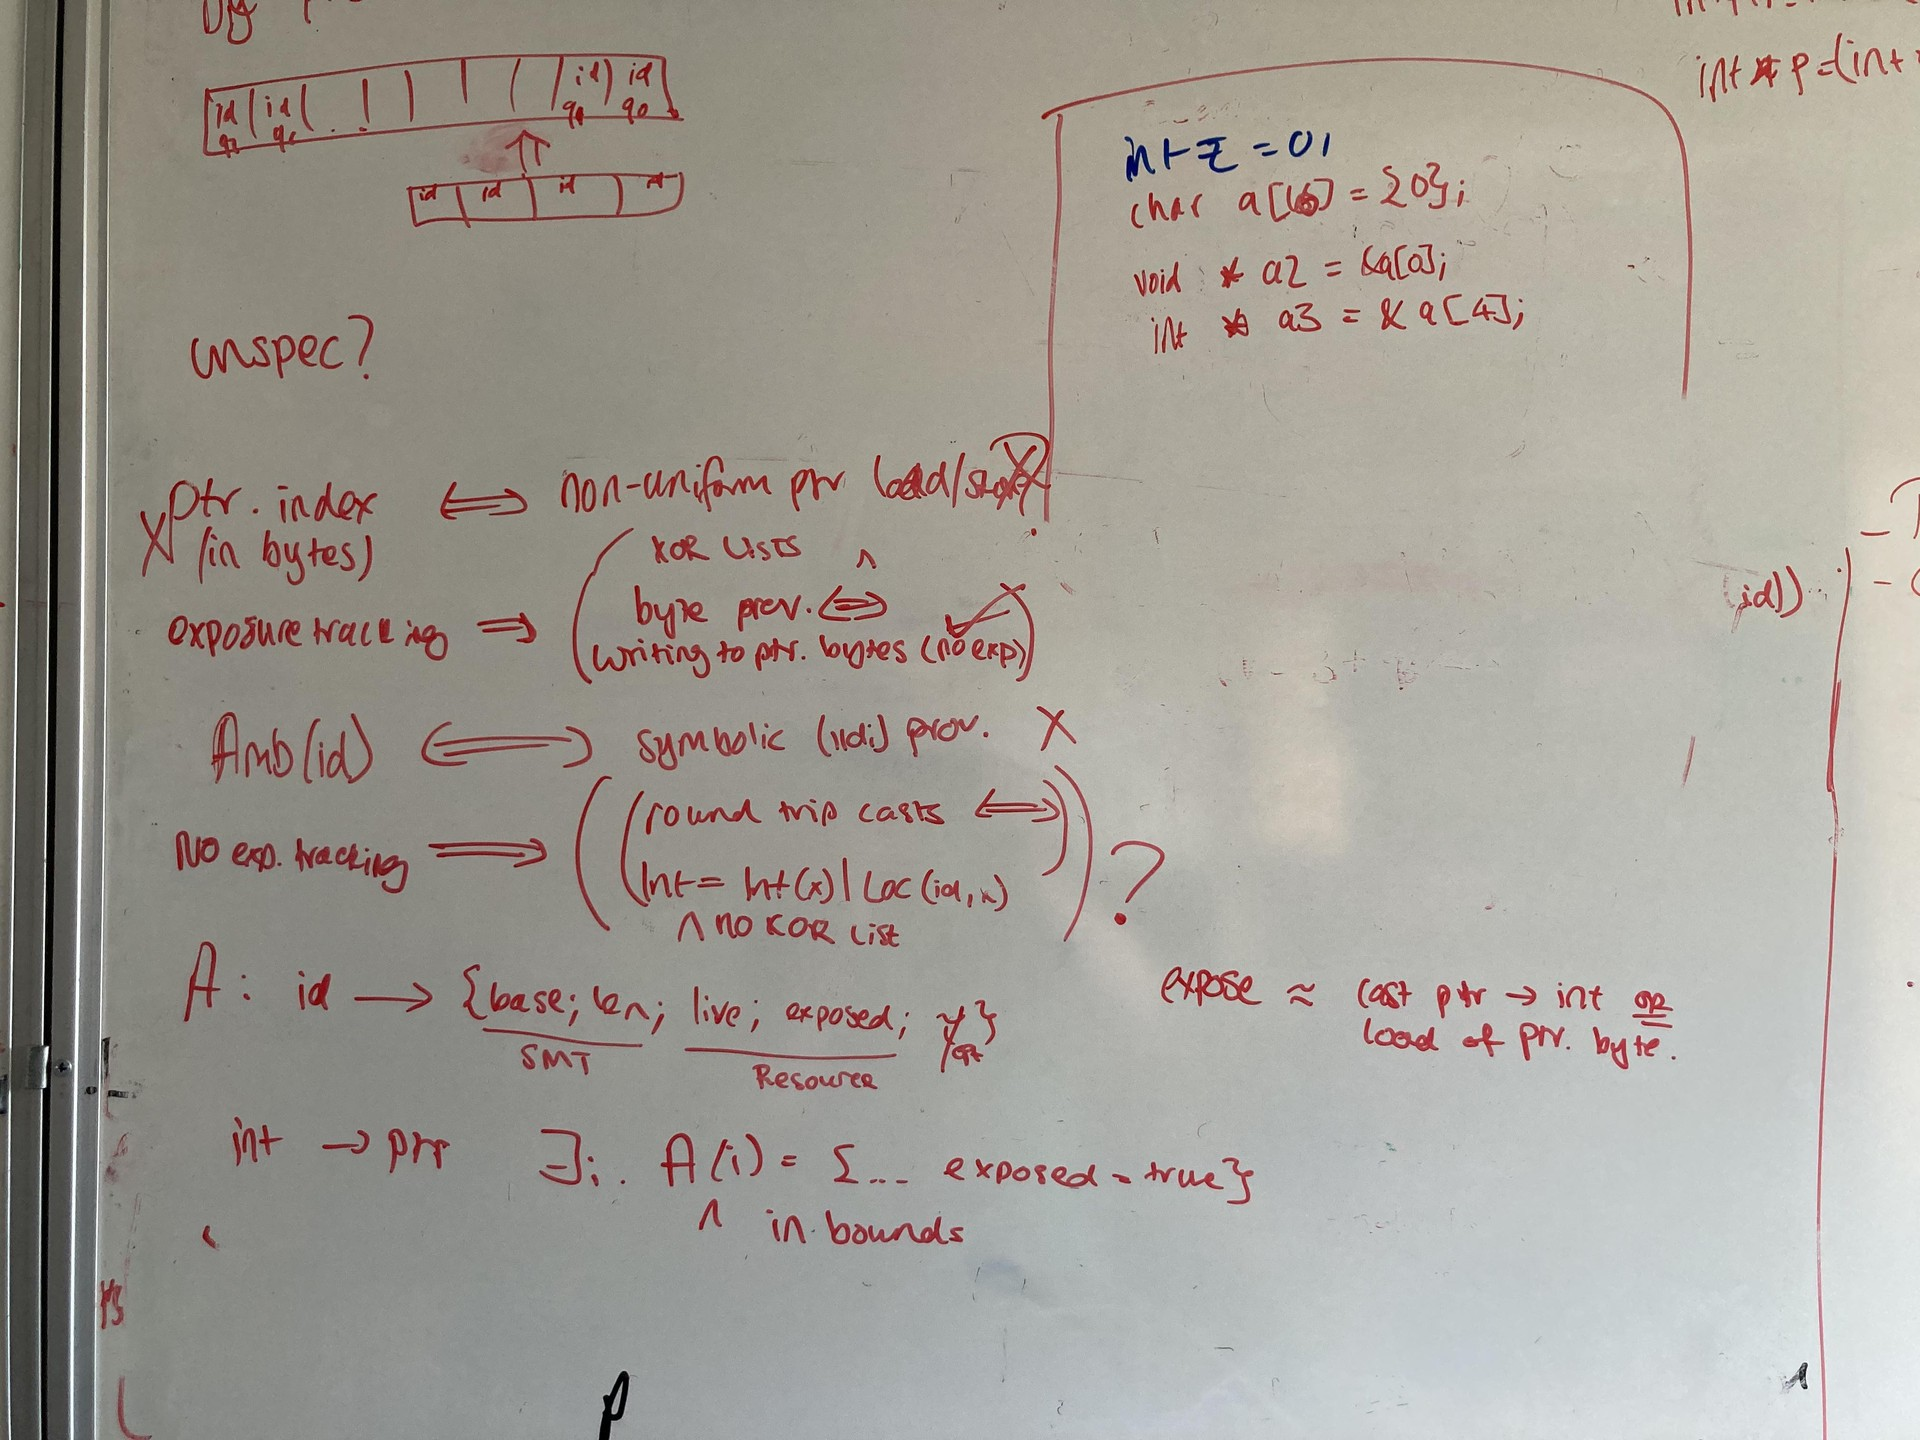
\includegraphics[width=\textwidth]{../misc/type-system-options.jpg}
\end{figure}

\section{CN-VIP}\label{sec:cn-vip}

\section{Soundness}\label{sec:cn-vip-soundness}

\section{Implementation}

Performance graph

\begin{figure}[h]
    \centering
    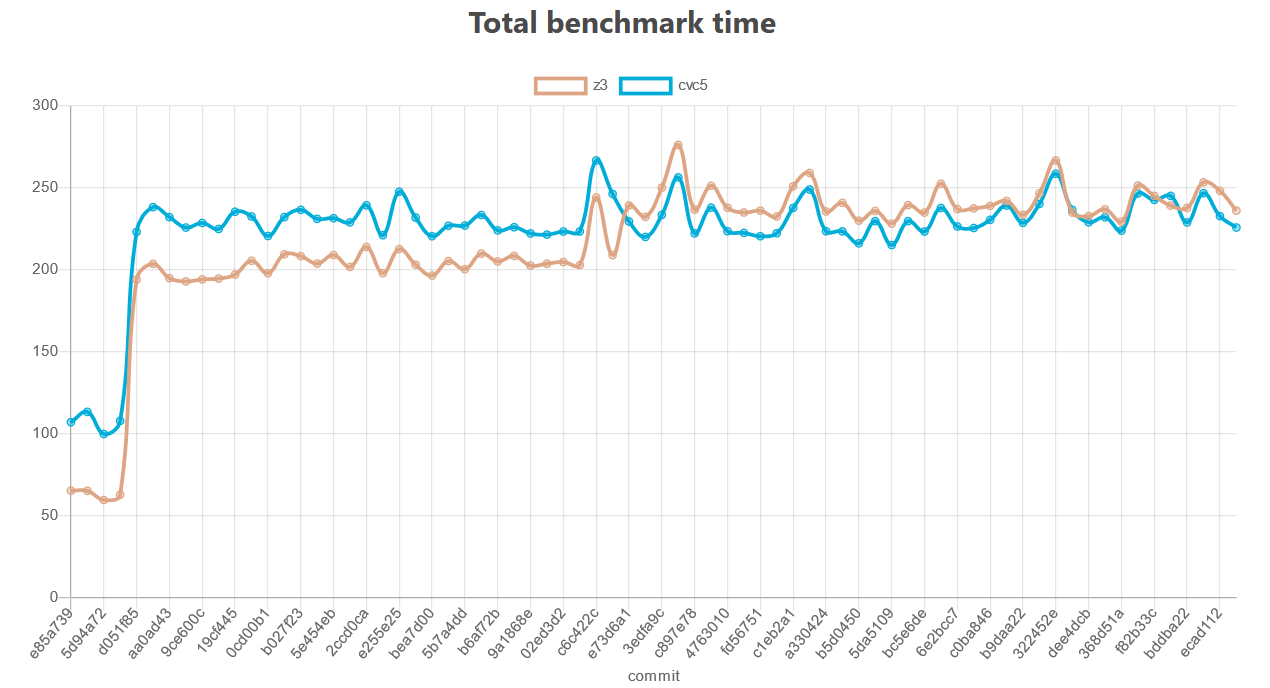
\includegraphics[width=\textwidth]{../misc/vip-performance-hit.png}
\end{figure}

\url{https://rems-project.githb.io/cerberus/dev/bench/}

\section{Translating resource lemmas}\label{sec:trans-res-lemmas}

Is there a reason, in the discussion about Cassia's PhD, we thought all of
Cerberus needed to be shoved into Iris instead of just a trace of memory model
(and eventually, concurrency) events?

irisification (cf
\url{https://people.mpi-sws.org/~dreyer/papers/iris-ground-up/paper.pdf}).  Either
just the resource algebra or (as DM suggests) also the abstract language of
memory model interface events: which one let one formalise the primitive
resource-context manipulations that CN does (conceivably extractably).

I think a sufficient halfway point would be the language of traces memory
events i.e.\ memory model as the dynamics. Resource algebra would be CN's view
of resources. Resource lemmas are then just statements saying that one resource
represents exactly the same heap as another resource (skips). Changes to the
resource algebra because of memory events (which we could introduce unsoundness
in CN) would be proved sound in Iris.

As a bonus, we could even formalise and prove sounds the inference procedures
CN uses (and with some engineering to handle SMT, even extract from Rocq).

The inference I'm talking about is resource context manipulations: checking if
we can pack or unpack predicates, if an owned is in the context, shifting
indices in and out of iterated predicates, exploding and imploding structs.
These operations don't require core structure.

Even if full extraction of the inference algo is not feasible (it would
involves standard data structures + SMT FFI), having a defined set of resource
manipulation primitives proved sound and extracting those (just standard data
structure manipulations), or even just proving the primitives sound and using a
similar interface would increase confidence.

If ones reads the above in reverse, it even provides a gradual migration path
which doesn't commit us to any next step and allows us to see how far
extraction can take us.

If the inference algs or the primitives are formalised, then we can iterate on
cleverer  inference schemes with a strong safety net

I think it will become more valuable as soon as we start having fancier things
like higher-order resources, locks, fractional permissions. At that point,
checking the steps/moves that any inference algorithm could take would get
closer to essential.

Even if an arbitrary inference algorithm is not stable, the steps available and
the shape of the resources should be more so, and that is worth at least
creating a clean abstraction for (and then pen-paper soundness, and then
mechanised soundness).

Noted and agreed that anything mechanised takes longer than one wants/expects
and that extraction is a pain. But this gives us a concrete use-case,
reasonable sequence of experiments and a clear idea of the benefits and costs.

